\documentclass[a4paper]{article}

\title{PH2255 Course:\\
Introduction to Statistical Methods\\Exercise 2}
\author{Thomas Bass}
\date{22 January 2021}

% LaTeX preambule: loading relevant packages, configuring Python listings
\usepackage{graphicx}
\usepackage{amsmath}
\usepackage{color}
\usepackage{listings}
\usepackage{hyperref}
\usepackage{bm}

\definecolor{dkgreen}{rgb}{0,0.6,0}
\definecolor{gray}{rgb}{0.5,0.5,0.5}
\definecolor{mauve}{rgb}{0.58,0,0.82}

% Settings for colour-coding and formatting Python code:
\lstset{
  language=Python,                % the language of the code
  basicstyle=\footnotesize,           % the size of the fonts that are used for the code
  numbers=left,                   % where to put the line-numbers
  numberstyle=\tiny\color{gray},  % the style that is used for the line-numbers
  stepnumber=5,                   % the step between two line-numbers. If it's 1, each line
                                  % will be numbered
  numbersep=5pt,                  % how far the line-numbers are from the code
  backgroundcolor=\color{white},      % choose the background color. You must add \usepackage{color}
  showspaces=false,               % show spaces adding particular underscores
  showstringspaces=false,         % underline spaces within strings
  showtabs=false,                 % show tabs within strings adding particular underscores
  frame=single,                   % adds a frame around the code
  rulecolor=\color{black},        % if not set, the frame-color may be changed on line-breaks within not-black text (e.g. commens (green here))
  tabsize=2,                      % sets default tabsize to 2 spaces
  captionpos=b,                   % sets the caption-position to bottom
  breaklines=true,                % sets automatic line breaking
  breakatwhitespace=false,        % sets if automatic breaks should only happen at whitespace
  title=\lstname,                   % show the filename of files included with \lstinputlisting;
                                  % also try caption instead of title
  keywordstyle=\color{blue},          % keyword style
  commentstyle=\color{dkgreen},       % comment style
  stringstyle=\color{mauve},         % string literal style
  escapeinside={\%*}{*)},            % if you want to add LaTeX within your code
  morekeywords={*,...}               % if you want to add more keywords to the set
}

\begin{document}
\maketitle

\begin{abstract}
Exercise Two in the PH2255 course introduces us to methods to quantify the "goodness-of-fit" of our curve fits generated last week using the method of minimising the sum of the squared residuals. By calculating the $\chi^2_\text{min}$ value for the parameters, we can use its ratio per the number of degrees of freedom to calculate the {\it p-value} for the fit, quantifying it's "goodness-of-fit".
\end{abstract}

\begin{figure}[b!]
\centerline{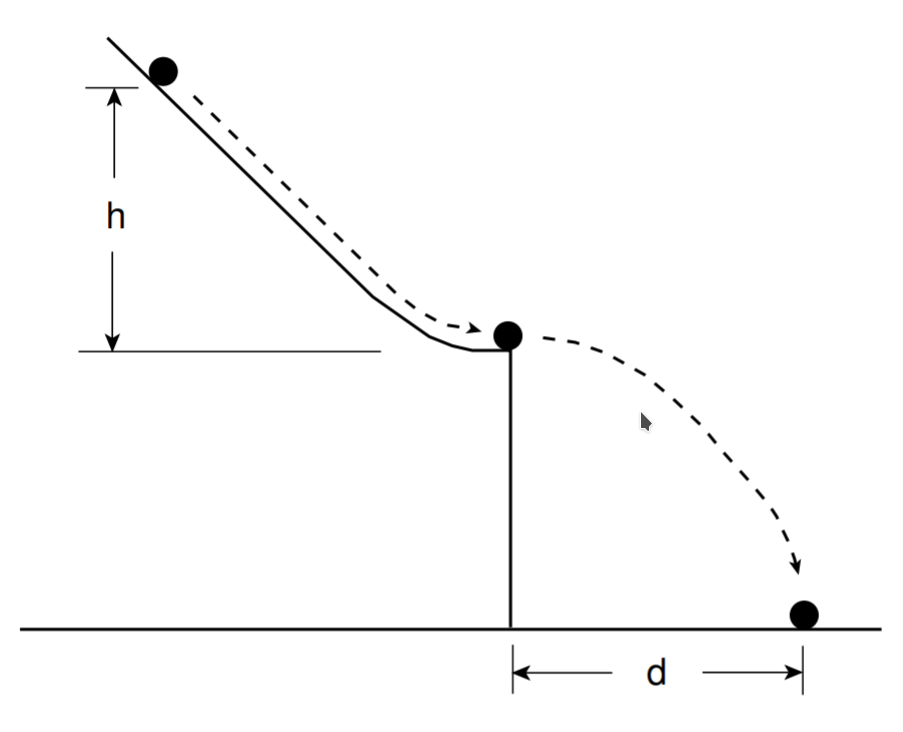
\includegraphics[scale=0.3]{experiment.png}}
\caption{The set-up that Galileo used for the ball and ramp experiment.}
\label{fig:experiment}
\end{figure}

For this exercise, we consider an historical experiment carried out by Galileo. The experiment involves, as shown in Figure \ref{fig:experiment}, rolling a ball down an inclined plane, where at the end of the ramp the trajectory is completely horizontal. The ball then rolls off the edge, and falls $H$ under projectile motion until it hits the ground, some horizontal distance $d$ away from the edge of the ramp. Galileo used the units {\it "punti"} to record his data: we assume one {\it punto} is around 1mm.

The data, taken from Galileo's journals, can be found in Table \ref{tab:table}. For this exercise, we assume an uncertainty of $\sigma = 15\text{punti}$ for all values of $d$, and a negligible uncertainty for $h$.

We can also include the data point of $(0, 0)$, as from a basic analysis we can conclude that if the ball fell from no height, it would have no velocity, and it would fall straight down to $d=0$.

The exercise instructs us to use two hypotheses for potential functional relationships between $d$ and $h$:
\begin{equation}
d=\alpha h
\end{equation}
\begin{equation}
d=\alpha h+\beta h^2
\end{equation}
\begin{equation}
d=\alpha h^\beta
\end{equation}

\begin{table}[t!]
\centering
\begin{tabular}{cc}
h & d\\ \hline\hline
1000 & 1500 \\
828  & 1340 \\
800  & 1328 \\
600  & 1172 \\
300  & 800  \\\hline
\end{tabular}
\caption{\label{tab:table}Data from Galileo's journal showing the horizontal distance $d$ of the ball before impact for five values of $h$}
\end{table}

Each of these equations, as well as the data used, was imported into Python with the following code:
\begin{lstlisting}
h   = np.array([1000., 828.,  800.,  600.,  300.])
d   = np.array([1500., 1340., 1328., 1172., 800.])
sig = np.array([15.,   15.,   15.,   15.,   15.])

# First hypothesis
def f1(h, *vars):
    a, = vars
    return a*h

# Second hypothesis
def f2(h, *vars):
    a, b = vars
    return a*h + b*h**2

# Third hypothesis
def f3(h, *vars):
    a, b = vars
    return a*h**b
\end{lstlisting}

For each of these hypotheses, we then carry out the least-squares fit from the previous exercise, using SciPy's \lstinline$curve_fit$ method, to generate the fitted parameters and their covariance matrices.
\newpage
\begin{lstlisting}
# Curve fitting
p0_1 = np.array([1.0])
theta_hat_1, covariance_1 = curve_fit(f1, h, d, p0_1, sig, absolute_sigma=True)

p0_2 = np.array([1.0, 1.0])
theta_hat_2, covariance_2 = curve_fit(f2, h, d, p0_2, sig, absolute_sigma=True)

p0_3 = np.array([1.0, 1.0])
theta_hat_3, covariance_3 = curve_fit(f3, h, d, p0_3, sig, absolute_sigma=True)

# Standard deviation of parameters
theta_hat_1_std_dev = np.sqrt(np.diag(covariance_1))

theta_hat_2_std_dev = np.sqrt(np.diag(covariance_2))

theta_hat_3_std_dev = np.sqrt(np.diag(covariance_3))
\end{lstlisting}
For each of these curve fits, we can produce plots:

\begin{figure}[h]
\centerline{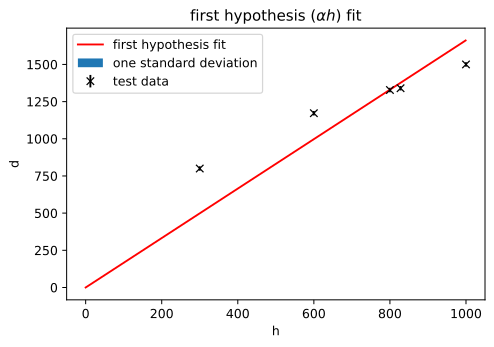
\includegraphics[scale=0.7]{h1.png}}
\caption{First hypothesis fit, showing fit curve and one standard deviation above and below}
\label{fig:fit1}
\end{figure}

\begin{figure}[htb!]
\centerline{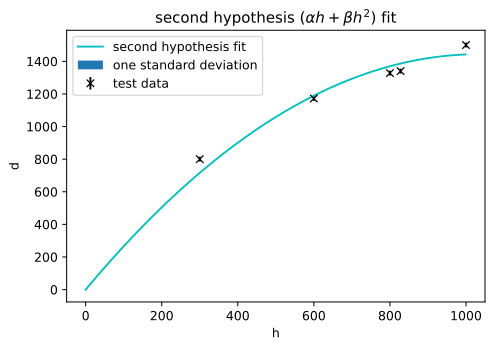
\includegraphics[scale=0.7]{h2.png}}
\caption{Second hypothesis fit, showing fit curve and one standard deviation above and below}
\label{fig:fit2}
\end{figure}

\begin{figure}[htb!]
\centerline{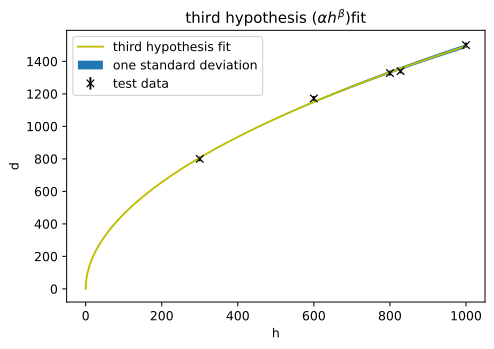
\includegraphics[scale=0.7]{h3.png}}
\caption{Third hypothesis fit, showing fit curve and one standard deviation above and below}
\label{fig:fit3}
\end{figure}
\newpage
Then, for each fit parameters, we can calculate the $\chi^2_\text{min}$ value. The equation, given as Equation 28 in the course handbook is:
\begin{equation} \label{eq:1}
\chi^2_\text{min}=\sum^N_{i=1}\frac{(y_i-f(x_i;\vec{\hat\theta}))^2}{\sigma^2_i}
\end{equation}
Converted into Python, as well as the calculation for the Degrees of Freedom, we get the following functions:
\newpage
\begin{lstlisting}
chi_sq_min = sum(((d - f1(h, *theta_hat))/sig)**2)
ndof = len(h)-len(p0)
\end{lstlisting}
SciPy's statistics module then provides us with a function to calculate the {\it p-value} from a given $\chi^2_\text{min}$ and number of degrees of freedom:
\begin{lstlisting}
p_val = scipy.stats.chi2.sf(chi_sq_min, df=ndof)
\end{lstlisting}
Using these functions on the calculated parameters from each fit, we get the following results:

\begin{table}[t!]
\centering
\begin{tabular}{ccc}
Hypothesis & $\chi^2_\text{min}$ & {\it p-value}\\ \hline\hline
$d=\alpha h$            & $165.50$ & $5.91\times10^{-142}$ \\
$d=\alpha h+\beta h^2$  & $21.58$  & $5.70\times10^{-14}$ \\
$d=\alpha h^\beta$      & $1.25$   & $0.29$  \\\hline
\end{tabular}
\caption{\label{tab:table}The $\chi^2_\text{min}$ values and {\it p-value}s obtained from each Hypothesis fit}
\end{table}

From these values, we can clearly conclude that the third hypothesis is the most accurate - the $\chi^2_\text{min}$ value is the closest to $1$, indicating that each value in the summation shown in Equation {\bf 4} is, on average, close to $1$, and therefore close to the actual provided data.

To verify this, we can use Newton's laws of motion to derive an actual equation relating $d$ to $h$, in terms of $h$, and the height of the edge of the ramp above the ground $H$. Using Conservation of Energy, we know that the total energy at the top of the ramp is equal to the total energy at the bottom of the ramp. The top of the ramp has Gravitational potential energy, and the bottom has Translational (kinetic) energy and rotational energy:

\begin{equation}
E_\text{gravitational}=E_\text{translation}+E_\text{rotation}
\end{equation}
\begin{equation}
mgh = \frac12mv^2 + \frac12I\omega^2
\end{equation}
Using the moment of inertia for a sphere $I=\frac25mr^2$:
\begin{equation}
mgh=\frac12mv^2+\frac12kmv^2
\end{equation}
Then, using projectile motion from the bottom of the ramp $d=vt$
\begin{equation}
mgh = \frac12m\left(\frac xt\right)^2 +\frac12 \frac25 m\left(\frac xt\right)^2
\end{equation}
\begin{equation}
\frac{x^2}{t^2}=10gh/7
\end{equation}
Then, using time of flight for the vertical drop under only the acceleration of gravity $H=\frac12gt^2$
\begin{equation}
d^2 = \left(\frac{10gh}{7}\right)\left(\frac H{\frac12g}\right)
\end{equation}
\begin{equation}
d=(10Hh/3.5)^\frac12
\end{equation}
If we set $\alpha=10H/3.5$ we get the equation $x=\alpha h^\frac12$. 

If we extract the exact values of $\alpha$ and $\beta$ from the $\vec{\hat\theta}$ values calculated in the curve fitting, we find $\alpha=43.76059028$ and $\beta=0.51105601$, giving us the empirical fitted equation:
\begin{equation}
d=43.76059028h^{0.51105601}
\end{equation}
The calculated value of $\beta$ in Equation {\bf 12} is sufficiently close to the predicted value of $0.5$ in Equation {\bf 11}, so we can conclude that the derived formula fits the actual data fitted by Hypothesis 3.

\begin{appendix}
\section{Python Code}\label{sec:python}
\lstinputlisting[language=Python,frame=single]{py.py}%
\begin{verbatim}
---Hypothesis 1---
Chi-sq-min/NDoF:	165.49753617897267
p-value:				 5.912867886616111e-142
---Hypothesis 2---
Chi-sq-min/NDoF:	21.58060512007567
p-value:				5.696198137767403e-14
---Hypothesis 3---
Chi-sq-min/NDoF:	1.2519761533914748
p-value:				0.2890541749901745
\end{verbatim}
\end{appendix}

\end{document}
